% Options for packages loaded elsewhere
\PassOptionsToPackage{unicode}{hyperref}
\PassOptionsToPackage{hyphens}{url}
%
\documentclass[
  ignorenonframetext,
]{beamer}
\usepackage{pgfpages}
\setbeamertemplate{caption}[numbered]
\setbeamertemplate{caption label separator}{: }
\setbeamercolor{caption name}{fg=normal text.fg}
\beamertemplatenavigationsymbolsempty
% Prevent slide breaks in the middle of a paragraph
\widowpenalties 1 10000
\raggedbottom
\setbeamertemplate{part page}{
  \centering
  \begin{beamercolorbox}[sep=16pt,center]{part title}
    \usebeamerfont{part title}\insertpart\par
  \end{beamercolorbox}
}
\setbeamertemplate{section page}{
  \centering
  \begin{beamercolorbox}[sep=12pt,center]{part title}
    \usebeamerfont{section title}\insertsection\par
  \end{beamercolorbox}
}
\setbeamertemplate{subsection page}{
  \centering
  \begin{beamercolorbox}[sep=8pt,center]{part title}
    \usebeamerfont{subsection title}\insertsubsection\par
  \end{beamercolorbox}
}
\AtBeginPart{
  \frame{\partpage}
}
\AtBeginSection{
  \ifbibliography
  \else
    \frame{\sectionpage}
  \fi
}
\AtBeginSubsection{
  \frame{\subsectionpage}
}

\usepackage{amsmath,amssymb}
\usepackage{iftex}
\ifPDFTeX
  \usepackage[T1]{fontenc}
  \usepackage[utf8]{inputenc}
  \usepackage{textcomp} % provide euro and other symbols
\else % if luatex or xetex
  \usepackage{unicode-math}
  \defaultfontfeatures{Scale=MatchLowercase}
  \defaultfontfeatures[\rmfamily]{Ligatures=TeX,Scale=1}
\fi
\usepackage{lmodern}
\usecolortheme{Flip}
\usefonttheme{serif} % use mainfont rather than sansfont for slide text
\useinnertheme{Flip}
\useoutertheme{Flip}
\ifPDFTeX\else  
    % xetex/luatex font selection
  \setmainfont[]{VisbyCF-Medium}
\fi
% Use upquote if available, for straight quotes in verbatim environments
\IfFileExists{upquote.sty}{\usepackage{upquote}}{}
\IfFileExists{microtype.sty}{% use microtype if available
  \usepackage[]{microtype}
  \UseMicrotypeSet[protrusion]{basicmath} % disable protrusion for tt fonts
}{}
\makeatletter
\@ifundefined{KOMAClassName}{% if non-KOMA class
  \IfFileExists{parskip.sty}{%
    \usepackage{parskip}
  }{% else
    \setlength{\parindent}{0pt}
    \setlength{\parskip}{6pt plus 2pt minus 1pt}}
}{% if KOMA class
  \KOMAoptions{parskip=half}}
\makeatother
\usepackage{xcolor}
\newif\ifbibliography
\setlength{\emergencystretch}{3em} % prevent overfull lines
\setcounter{secnumdepth}{-\maxdimen} % remove section numbering


\providecommand{\tightlist}{%
  \setlength{\itemsep}{0pt}\setlength{\parskip}{0pt}}\usepackage{longtable,booktabs,array}
\usepackage{calc} % for calculating minipage widths
\usepackage{caption}
% Make caption package work with longtable
\makeatletter
\def\fnum@table{\tablename~\thetable}
\makeatother
\usepackage{graphicx}
\makeatletter
\def\maxwidth{\ifdim\Gin@nat@width>\linewidth\linewidth\else\Gin@nat@width\fi}
\def\maxheight{\ifdim\Gin@nat@height>\textheight\textheight\else\Gin@nat@height\fi}
\makeatother
% Scale images if necessary, so that they will not overflow the page
% margins by default, and it is still possible to overwrite the defaults
% using explicit options in \includegraphics[width, height, ...]{}
\setkeys{Gin}{width=\maxwidth,height=\maxheight,keepaspectratio}
% Set default figure placement to htbp
\makeatletter
\def\fps@figure{htbp}
\makeatother

\usepackage{tabu}
\makeatletter
\makeatother
\makeatletter
\makeatother
\makeatletter
\@ifpackageloaded{caption}{}{\usepackage{caption}}
\AtBeginDocument{%
\ifdefined\contentsname
  \renewcommand*\contentsname{Table of contents}
\else
  \newcommand\contentsname{Table of contents}
\fi
\ifdefined\listfigurename
  \renewcommand*\listfigurename{List of Figures}
\else
  \newcommand\listfigurename{List of Figures}
\fi
\ifdefined\listtablename
  \renewcommand*\listtablename{List of Tables}
\else
  \newcommand\listtablename{List of Tables}
\fi
\ifdefined\figurename
  \renewcommand*\figurename{Figure}
\else
  \newcommand\figurename{Figure}
\fi
\ifdefined\tablename
  \renewcommand*\tablename{Table}
\else
  \newcommand\tablename{Table}
\fi
}
\@ifpackageloaded{float}{}{\usepackage{float}}
\floatstyle{ruled}
\@ifundefined{c@chapter}{\newfloat{codelisting}{h}{lop}}{\newfloat{codelisting}{h}{lop}[chapter]}
\floatname{codelisting}{Listing}
\newcommand*\listoflistings{\listof{codelisting}{List of Listings}}
\makeatother
\makeatletter
\@ifpackageloaded{caption}{}{\usepackage{caption}}
\@ifpackageloaded{subcaption}{}{\usepackage{subcaption}}
\makeatother
\makeatletter
\@ifpackageloaded{tcolorbox}{}{\usepackage[skins,breakable]{tcolorbox}}
\makeatother
\makeatletter
\@ifundefined{shadecolor}{\definecolor{shadecolor}{rgb}{.97, .97, .97}}
\makeatother
\makeatletter
\makeatother
\makeatletter
\makeatother
\ifLuaTeX
  \usepackage{selnolig}  % disable illegal ligatures
\fi
\IfFileExists{bookmark.sty}{\usepackage{bookmark}}{\usepackage{hyperref}}
\IfFileExists{xurl.sty}{\usepackage{xurl}}{} % add URL line breaks if available
\urlstyle{same} % disable monospaced font for URLs
\hypersetup{
  pdftitle={Analyse exploratoire},
  pdfauthor={Léo Belzile},
  hidelinks,
  pdfcreator={LaTeX via pandoc}}

\title{Analyse exploratoire}
\subtitle{Analyse multidimensionnelle appliquée}
\author{Léo Belzile}
\date{}
\institute{HEC Montréal}

\begin{document}
\frame{\titlepage}
\ifdefined\Shaded\renewenvironment{Shaded}{\begin{tcolorbox}[frame hidden, sharp corners, interior hidden, borderline west={3pt}{0pt}{shadecolor}, breakable, enhanced, boxrule=0pt]}{\end{tcolorbox}}\fi

\begin{frame}{Analyse de données}
\protect\hypertarget{analyse-de-donnuxe9es}{}
\begin{figure}

{\centering 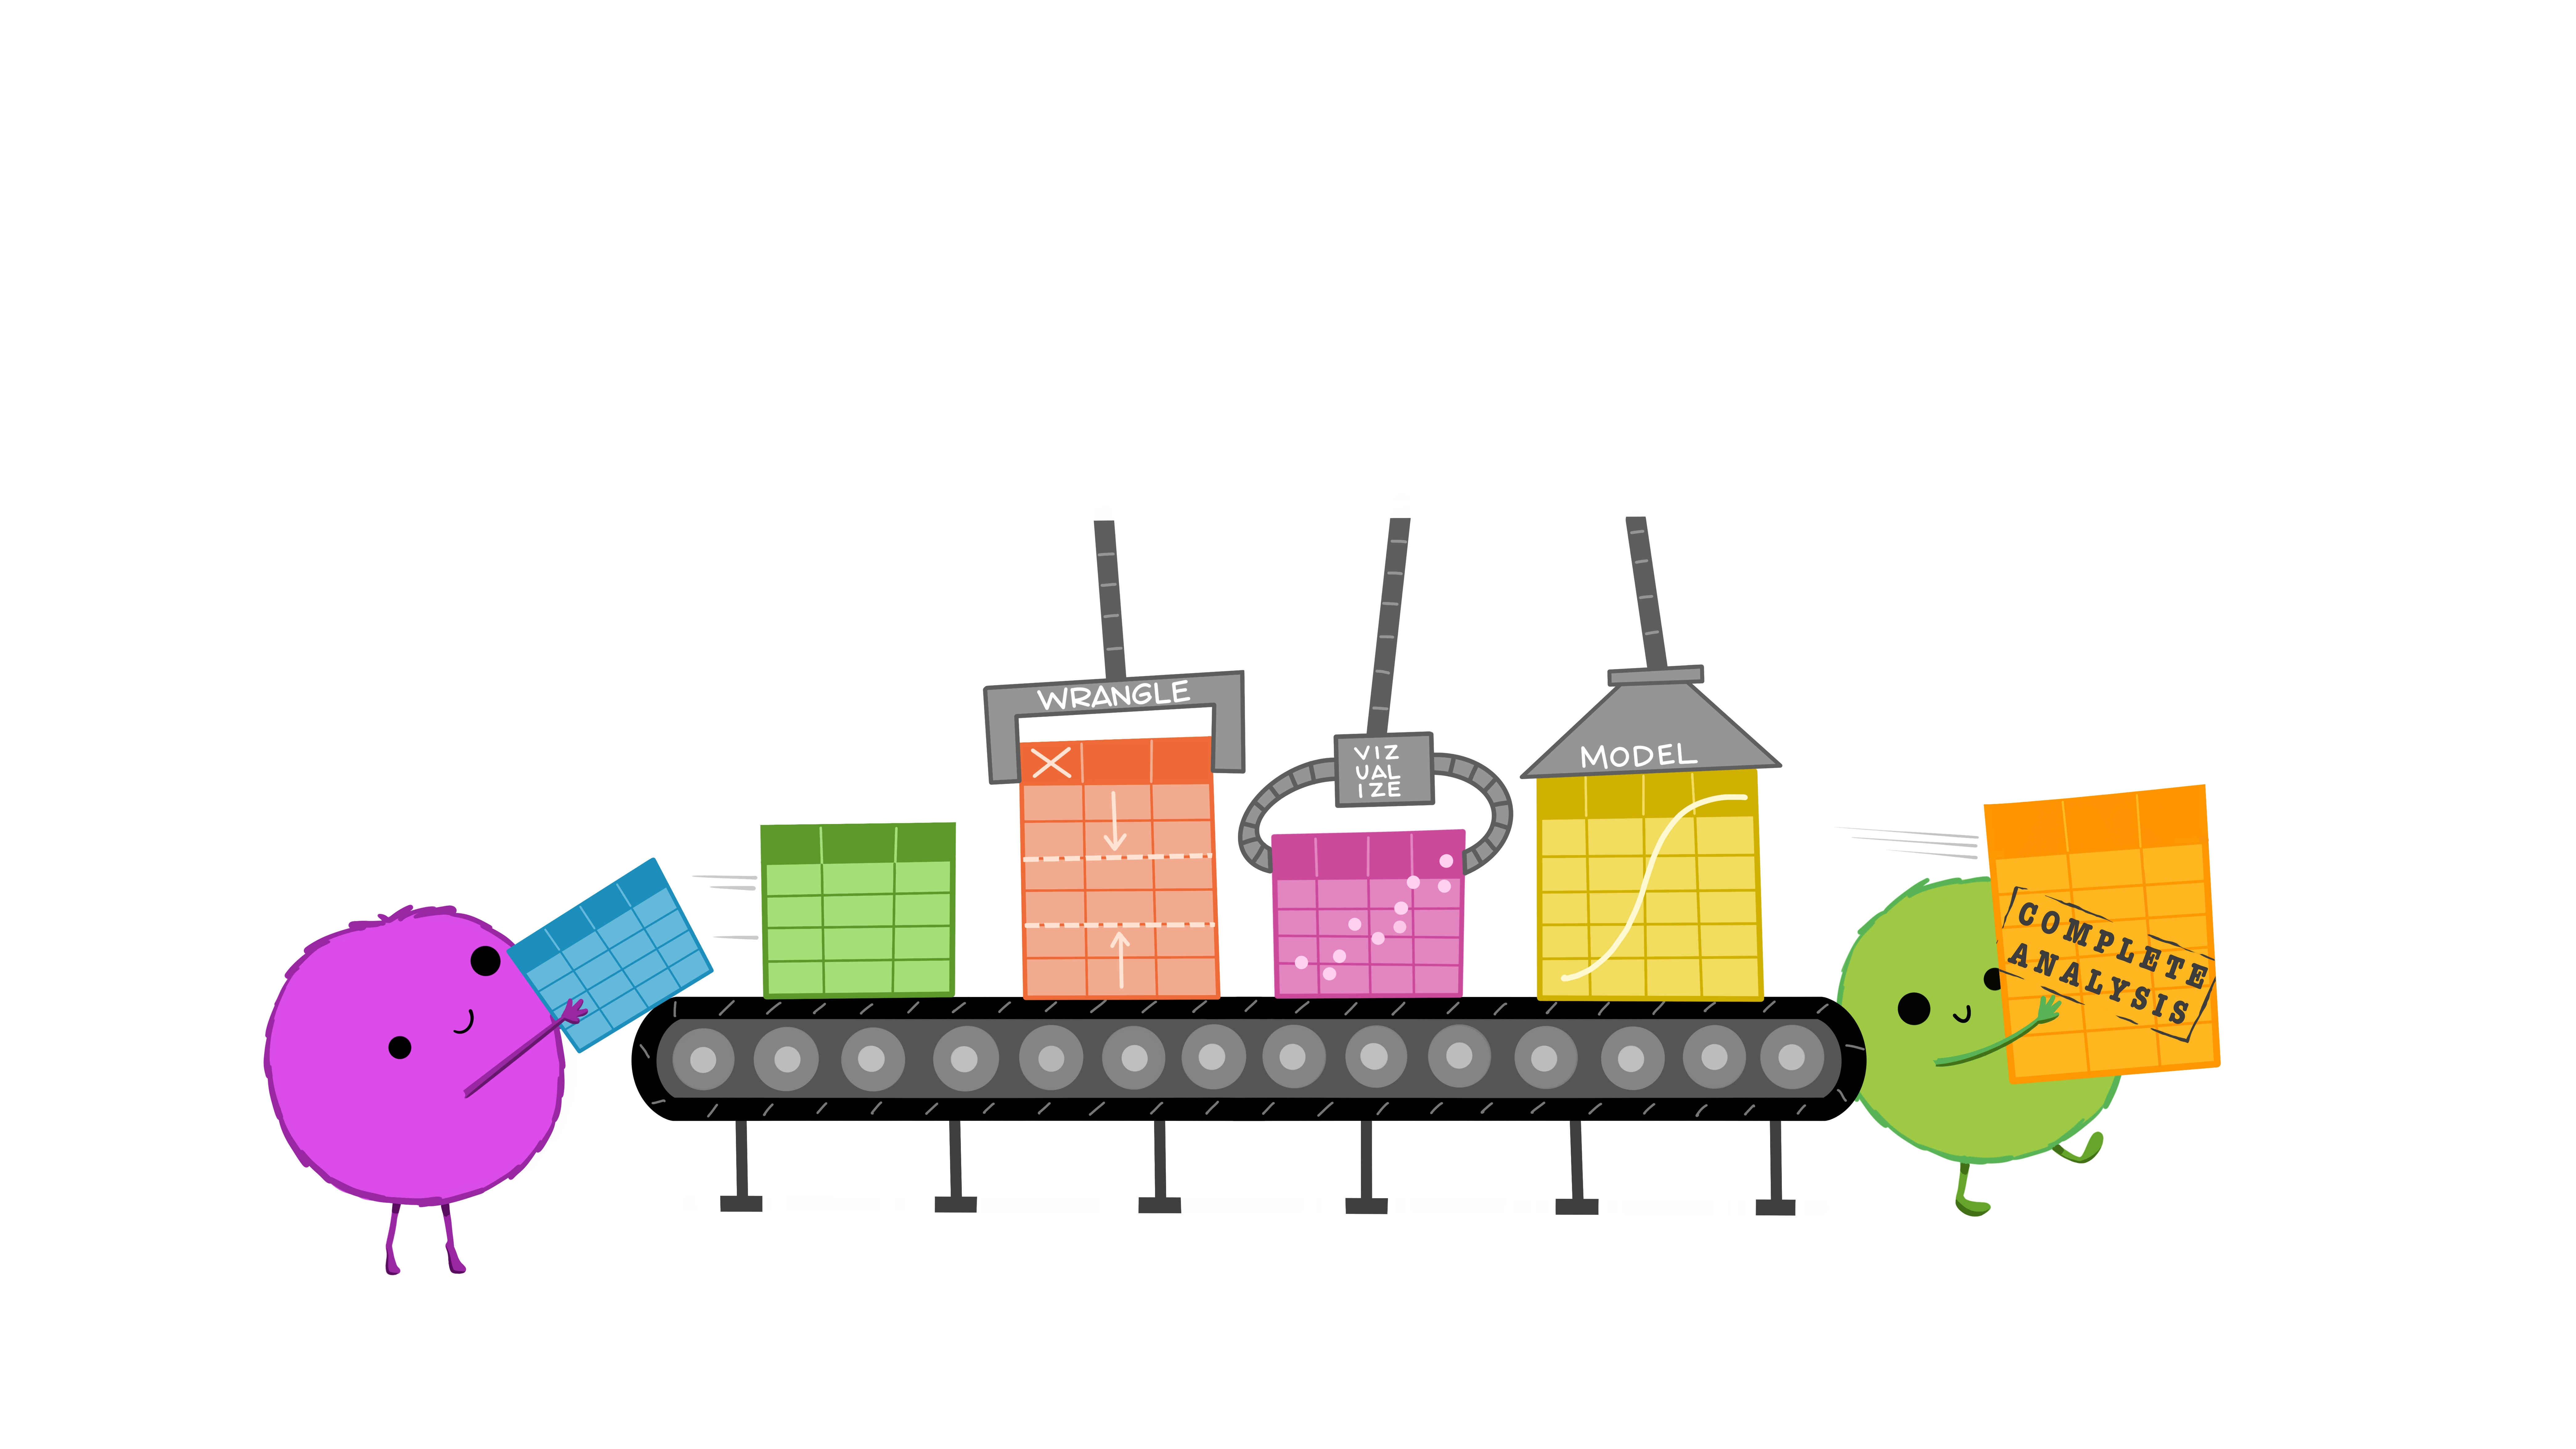
\includegraphics[width=1\textwidth,height=\textheight]{figures/tidydata_5.jpg}

}

\caption{Allison Horst (CC BY 4.0)}

\end{figure}
\end{frame}

\begin{frame}{Organisation du travail}
\protect\hypertarget{organisation-du-travail}{}
\begin{figure}

{\centering 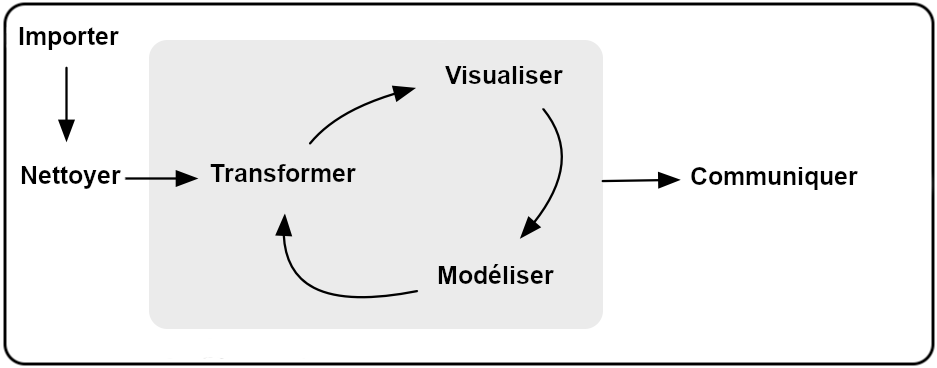
\includegraphics[width=0.9\textwidth,height=\textheight]{figures/r4ds_data-science_fr.png}

}

\caption{Adapté de \emph{R for Data Science}, H. Wickham et G.
Grolemund}

\end{figure}
\end{frame}

\begin{frame}{Organisation des données}
\protect\hypertarget{organisation-des-donnuxe9es}{}
\textbf{Quelques bonnes pratiques}

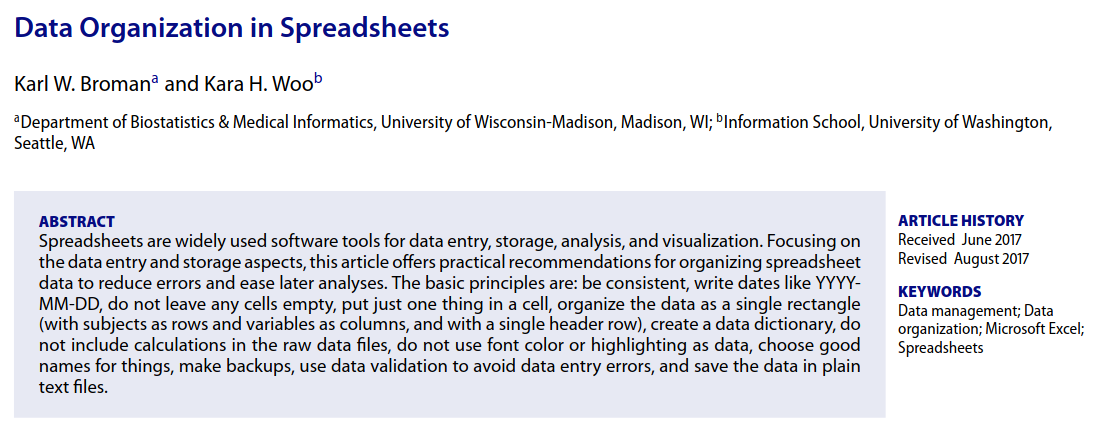
\includegraphics{figures/DataOrganizationinSpreadsheets.png}

\begin{quote}
Karl W. Broman \& Kara H. Woo (2018) Data Organization in Spreadsheets,
The American Statistician, 72:1, 2-10, DOI:
10.1080/00031305.2017.1375989
\end{quote}
\end{frame}

\begin{frame}{Nettoyage des données}
\protect\hypertarget{nettoyage-des-donnuxe9es}{}
\begin{itemize}
\tightlist
\item
  Toujours garder une copie des données brutes
\item
  Automatiser le nettoyage
\end{itemize}

\includegraphics{MATH60602-diapos1_files/figure-beamer/unnamed-chunk-3-1.pdf}

Ne jamais ouvrir et modifier/sauvegarder les données dans Excel!
\end{frame}

\begin{frame}{Histoires d'horreur}
\protect\hypertarget{histoires-dhorreur}{}
\begin{figure}

{\centering 
\includegraphics[width=0.9\textwidth,height=\textheight]{figures/guardian-covid-excel.png}

}

\caption{Capture d'écran d'un article du quotidien \emph{The Guardian}}

\end{figure}
\end{frame}

\begin{frame}{Données en format ``tidy''}
\protect\hypertarget{donnuxe9es-en-format-tidy}{}
\begin{itemize}
\tightlist
\item
  variables en colonnes
\item
  observations en lignes
\item
  une seule mesure par cellule
\end{itemize}

\begin{figure}

{\centering 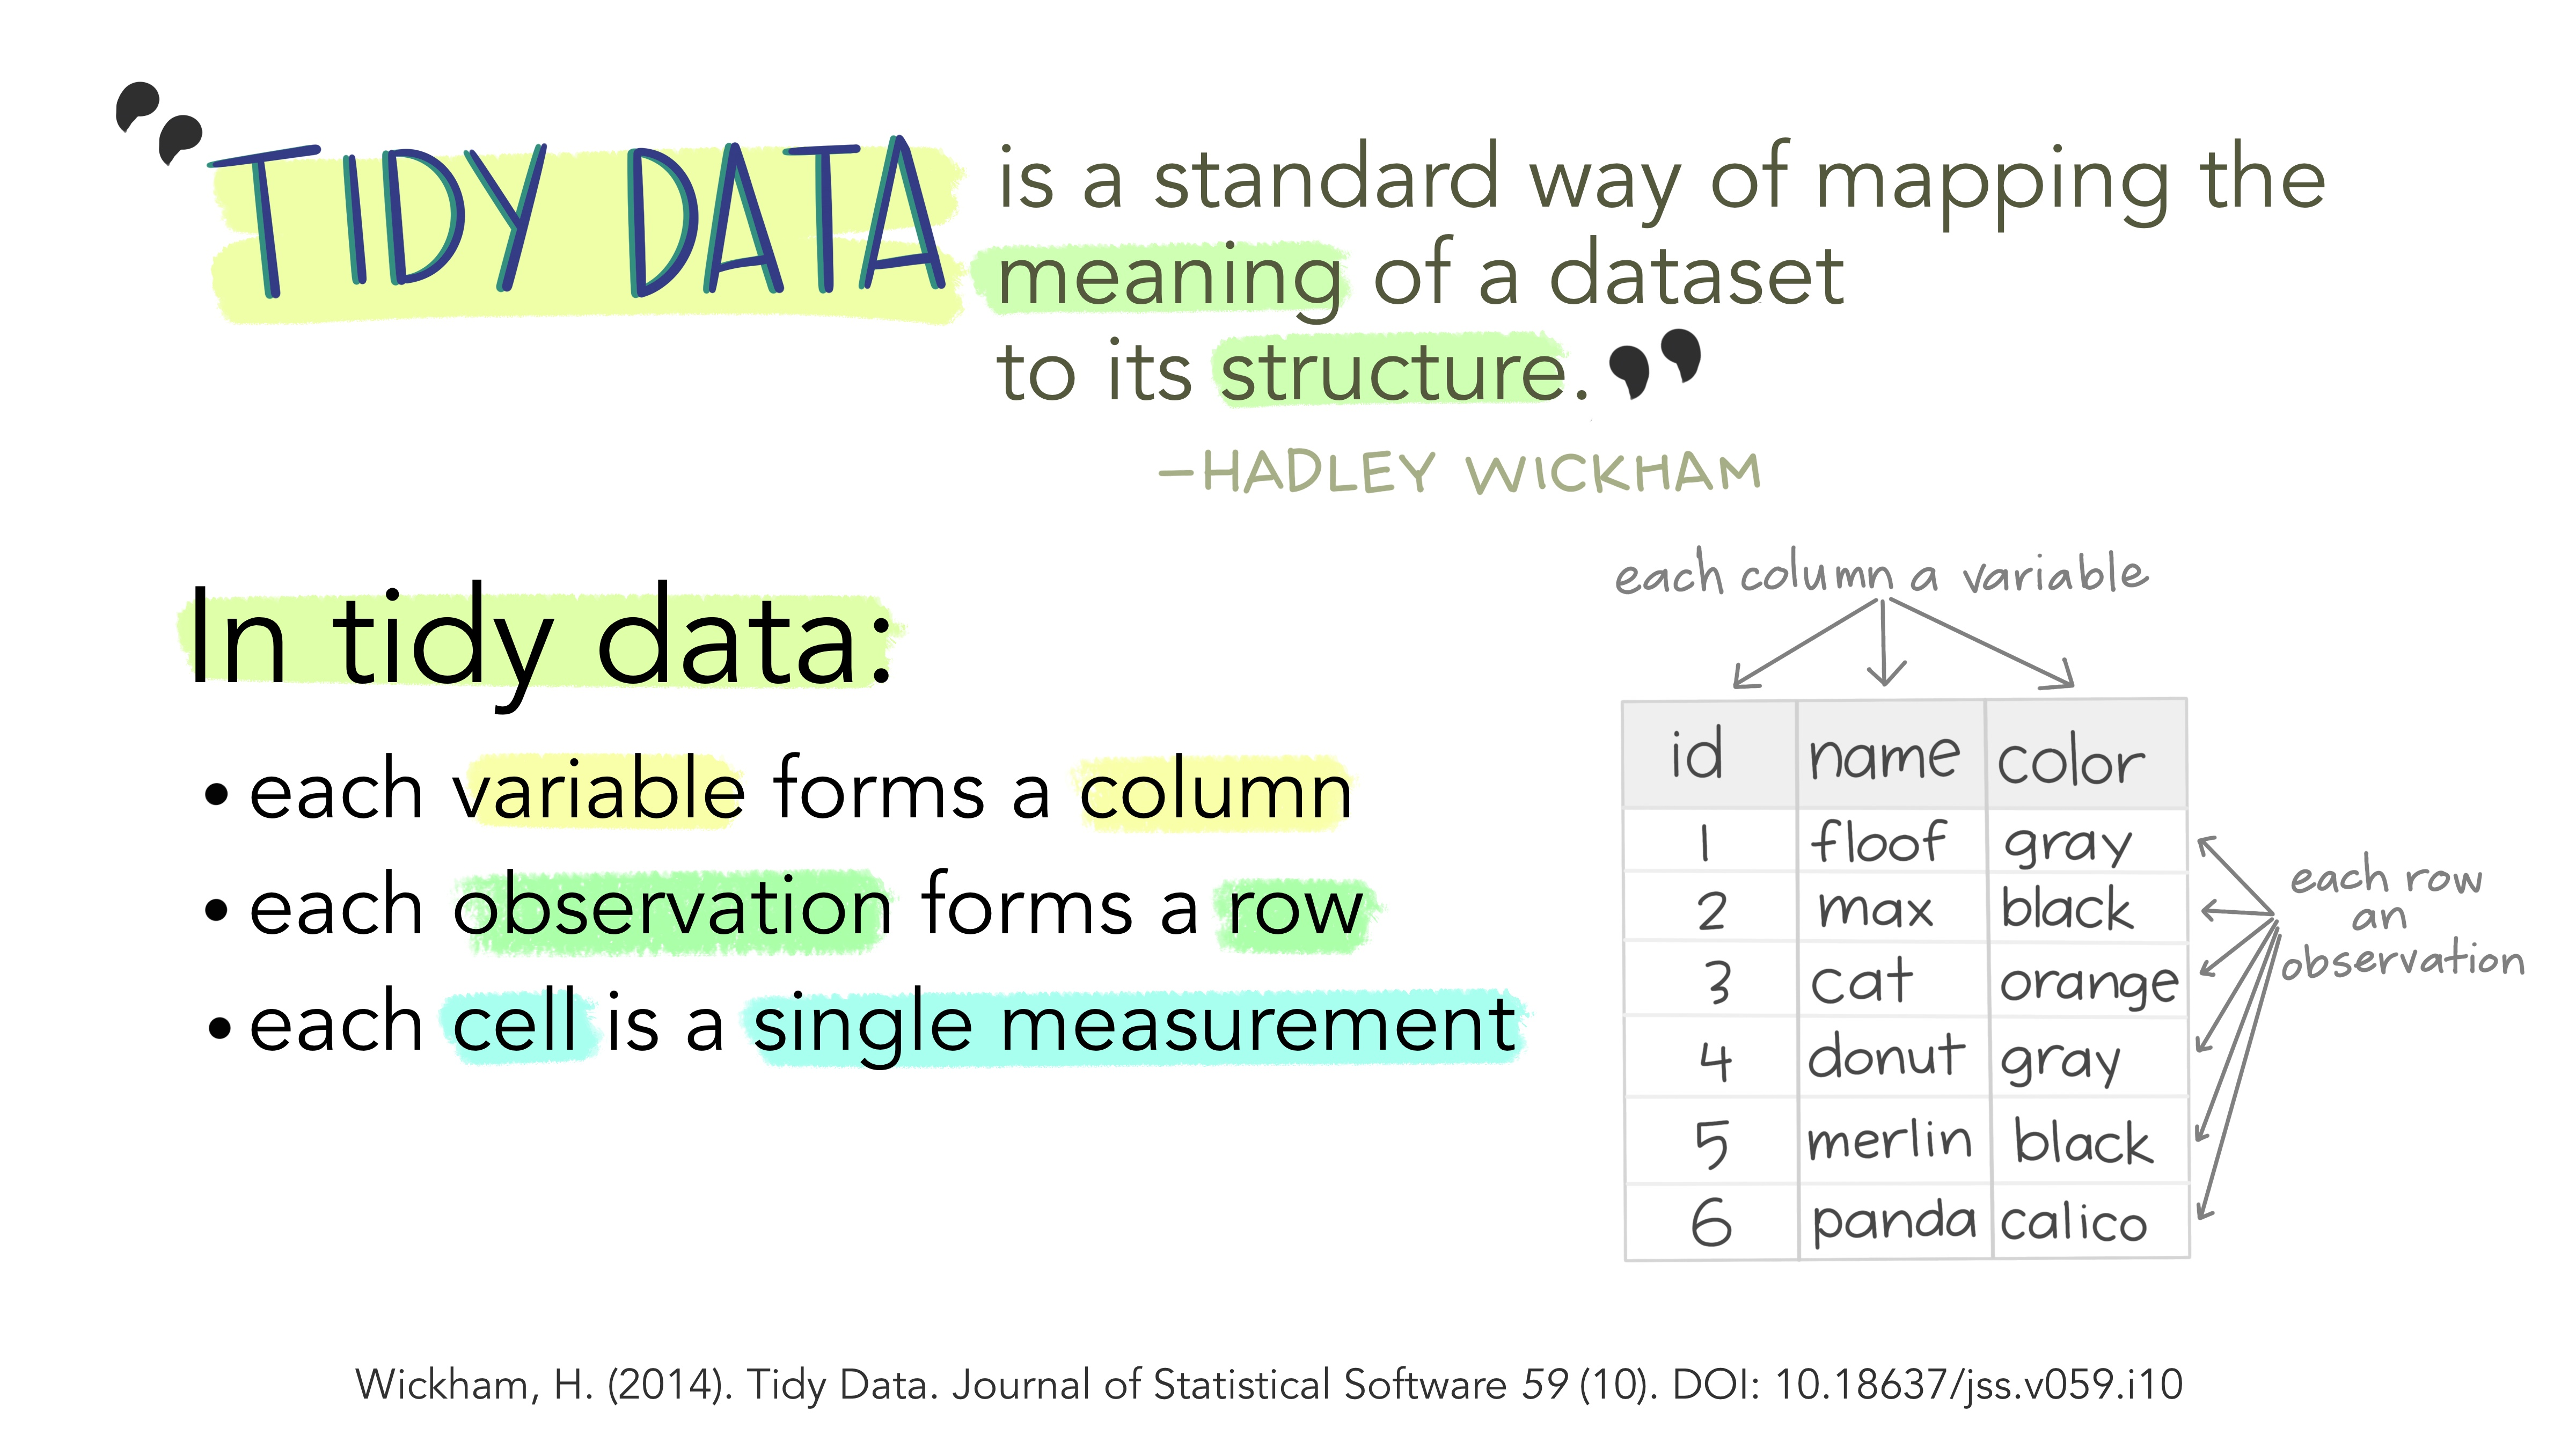
\includegraphics[width=0.7\textwidth,height=\textheight]{figures/tidydata_1.jpg}

}

\caption{Allison Horst (CC BY 4.0)}

\end{figure}
\end{frame}

\begin{frame}{Exemple}
\protect\hypertarget{exemple}{}
Est-ce que ces données de la Régie de l'Énergie sont en format `tidy'?

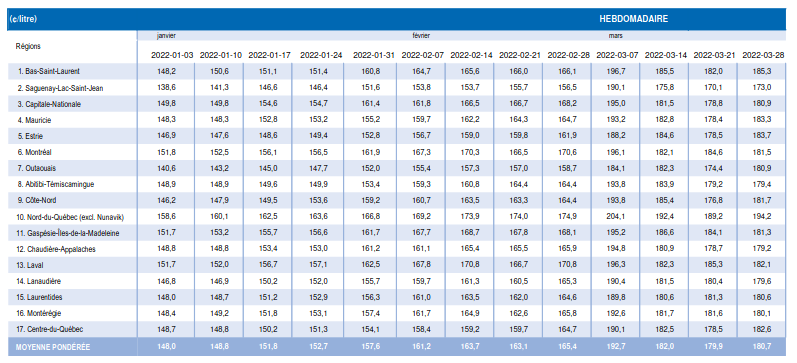
\includegraphics[width=1\textwidth,height=\textheight]{figures/regie-energie.png}
\end{frame}

\begin{frame}{Types de variables numériques}
\protect\hypertarget{types-de-variables-numuxe9riques}{}
\begin{figure}

{\centering 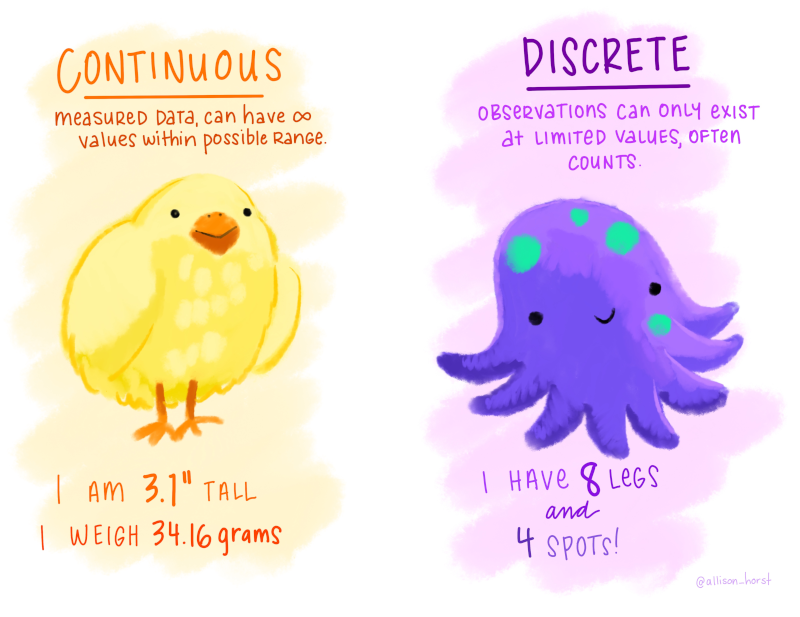
\includegraphics[width=0.8\textwidth,height=\textheight]{figures/continuous_discrete.png}

}

\caption{Allison Horst (CC BY 4.0)}

\end{figure}
\end{frame}

\begin{frame}{Types de variables catégorielles}
\protect\hypertarget{types-de-variables-catuxe9gorielles}{}
\begin{figure}

{\centering 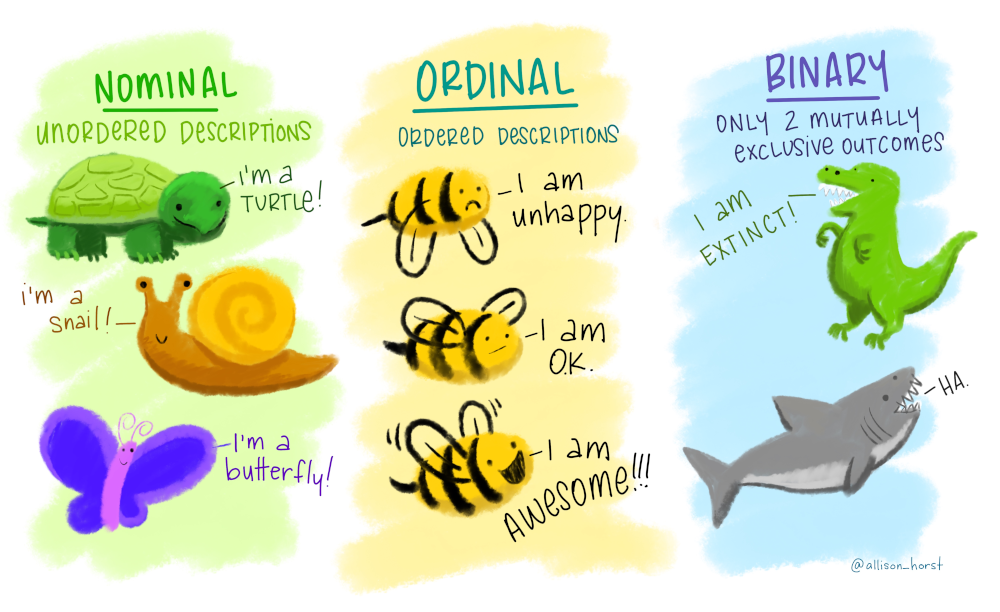
\includegraphics[width=0.8\textwidth,height=\textheight]{figures/nominal_ordinal_binary.png}

}

\caption{Allison Horst (CC BY 4.0)}

\end{figure}
\end{frame}

\begin{frame}[fragile]{Validation des données}
\protect\hypertarget{validation-des-donnuxe9es}{}
Vérifier la présence de

\begin{itemize}
\tightlist
\item
  valeurs manquantes (\texttt{NA}, points, cellules vides, 999, -1,
  etc.)
\item
  relations logiques (total, moyenne, etc.) entre variables
\item
  variables catégorielles non déclarées

  \begin{itemize}
  \tightlist
  \item
    valeur entière (par ex., jours de la semaine)
  \item
    chaînes de caractère
  \end{itemize}
\end{itemize}
\end{frame}

\begin{frame}{Visualisation}
\protect\hypertarget{visualisation}{}
\begin{quote}
\emph{Un simple graphique transmet plus d'information à l'analyste que
n'importe quel autre option}
\end{quote}

\begin{columns}[T]
\begin{column}{0.8\textwidth}
\end{column}

\begin{column}{0.2\textwidth}
John Tukey
\end{column}
\end{columns}
\end{frame}

\begin{frame}{Qu'est ce qu'un bon graphique?}
\protect\hypertarget{quest-ce-quun-bon-graphique}{}
\begin{quote}
\emph{communique des idées complexes avec clarté, précision et
efficacité \ldots{} le graphique qui offre au lecteur le plus grand
nombre d'idées le plus rapidement possible avec le moins d'encre et le
plus petit espace possible}
\end{quote}

\begin{columns}[T]
\begin{column}{0.7\textwidth}
\end{column}

\begin{column}{0.3\textwidth}
Edward Tufte, 1983
\end{column}
\end{columns}
\end{frame}

\begin{frame}{Grammaire des graphiques}
\protect\hypertarget{grammaire-des-graphiques}{}
\begin{columns}[T]
\begin{column}{0.4\textwidth}
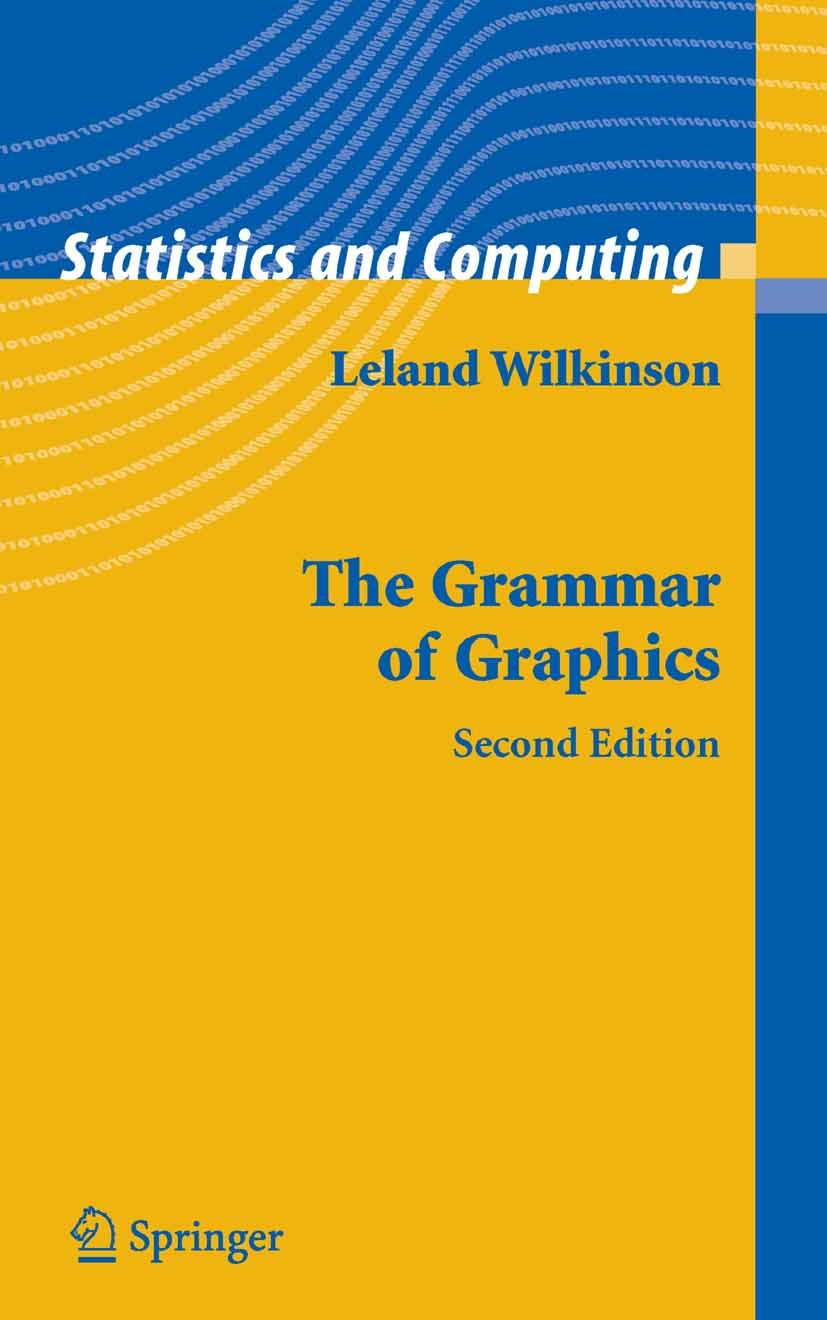
\includegraphics[width=0.8\textwidth,height=\textheight]{img/03/gg-book.jpg}
\end{column}

\begin{column}{0.6\textwidth}
\begin{itemize}
\tightlist
\item
  Éléments (couches):

  \begin{itemize}
  \tightlist
  \item
    données
  \item
    application (variable \(\to\) esthétique)
  \item
    objets géométriques
  \item
    transformations
  \item
    positionnement
  \end{itemize}
\item
  Échelle / guide
\item
  Coordonnées (facettes, système de coordonnés)
\end{itemize}
\end{column}
\end{columns}
\end{frame}

\begin{frame}{Règles d'or}
\protect\hypertarget{ruxe8gles-dor}{}
Pour une visualisation effective:

\begin{enumerate}
\tightlist
\item
  le choix du graphique dépend du type de variable
\item
  soignez les apparences
\item
  portez une attention particulière à la perception visuelle humaine
\end{enumerate}
\end{frame}

\begin{frame}{Règle 1: choix de graphiques avec une seule variable}
\protect\hypertarget{ruxe8gle-1-choix-de-graphiques-avec-une-seule-variable}{}
\begin{itemize}
\tightlist
\item
  continue: histogramme, densité
\item
  discrète: diagramme en bâton
\item
  catégorielle: diagramme en bâton (fréquence ou pourcentage)
\end{itemize}
\end{frame}

\begin{frame}
\begin{figure}

{\centering \includegraphics{MATH60602-diapos1_files/figure-beamer/figure-renfe_barplot-1.pdf}

}

\end{figure}
\end{frame}

\begin{frame}
\begin{figure}

{\centering \includegraphics{MATH60602-diapos1_files/figure-beamer/renfe_hist-1.png}

}

\end{figure}
\end{frame}

\begin{frame}{Règle 1: choix de graphiques avec deux variables}
\protect\hypertarget{ruxe8gle-1-choix-de-graphiques-avec-deux-variables}{}
\begin{itemize}
\tightlist
\item
  continues: nuage de points
\item
  catégorielles: diagramme à bande (avec couleurs), carte thermique
\item
  continue \(\times\) catégorielle: boîte à moustache, graphique violon
\end{itemize}
\end{frame}

\begin{frame}{Boîte à moustaches}
\protect\hypertarget{bouxeete-uxe0-moustaches}{}
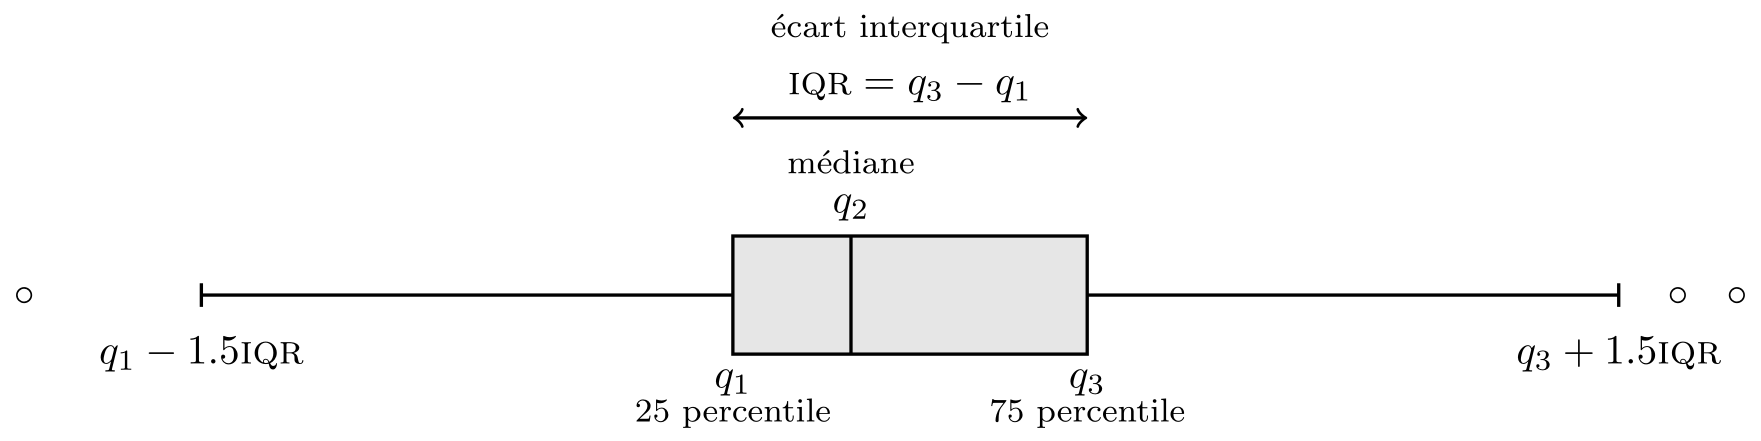
\includegraphics[width=1\textwidth,height=\textheight]{figures/01-intro-boiteamoustache.png}
\end{frame}

\begin{frame}
\begin{figure}

{\centering \includegraphics[width=1\textwidth,height=\textheight]{MATH60602-diapos1_files/figure-beamer/renfe_boxplot-1.png}

}

\end{figure}
\end{frame}

\begin{frame}
\begin{figure}

{\centering \includegraphics[width=0.7\textwidth,height=\textheight]{MATH60602-diapos1_files/figure-beamer/renfe_nuagepts_code-1.png}

}

\end{figure}

\begin{itemize}
\tightlist
\item
  Qu'est-ce qui cloche dans la représentation graphique précédente?
\item
  Comment pourrait-on remédier aux problèmes soulevés?
\end{itemize}
\end{frame}

\begin{frame}{Règle 2: soignez les apparences}
\protect\hypertarget{ruxe8gle-2-soignez-les-apparences}{}
Certaines visualisations sont plus effectives/adéquates que d'autres

\begin{itemize}
\tightlist
\item
  votre graphique doit être interprétable uniquement avec la légende.
\item
  inclure les noms de variables \textbf{et} les unités
\item
  ajouter une description dans le texte et faire une référence croisée
\end{itemize}
\end{frame}

\begin{frame}{Éléments graphiques clés}
\protect\hypertarget{uxe9luxe9ments-graphiques-cluxe9s}{}
\begin{itemize}
\tightlist
\item
  Titre et annotation
\item
  Libellés et unités sur les axes
\item
  Libellé de l'axe des \(y\) en sous-titre
\item
  Inverser les axes si les étiquettes trop longue (variable
  catégorielles)
\end{itemize}
\end{frame}

\begin{frame}{Règle 3: perception visuelle humaine}
\protect\hypertarget{ruxe8gle-3-perception-visuelle-humaine}{}
\begin{itemize}
\tightlist
\item
  ratio longueur/largeur
\item
  taille de police suffisante pour lisibilité
\item
  espace entre bandes
\item
  étendu des axes (incluant ou pas zéro)
\item
  choix de couleurs

  \begin{itemize}
  \tightlist
  \item
    noir/blanc avec contraste
  \item
    palettes pour daltoniens
  \end{itemize}
\item
  comparaison d'aires/superficies (difficile)
\item
  graphiques 3D / avec rotation superflue à éviter
\end{itemize}
\end{frame}

\begin{frame}{Problèmes de perceptions}
\protect\hypertarget{probluxe8mes-de-perceptions}{}
\includegraphics{MATH60602-diapos1_files/figure-beamer/unnamed-chunk-13-1.pdf}
\end{frame}

\begin{frame}{Mauvaise palette de couleur}
\protect\hypertarget{mauvaise-palette-de-couleur}{}
\begin{itemize}
\item
  Gauche: Carte originale de la NOAA en niveaux de gris: on voit
  clairement le problème de saturation
\item
  Droite: solution potentielle avec palette de couleurs différente.
\end{itemize}

\includegraphics{MATH60602-diapos1_files/figure-beamer/unnamed-chunk-14-1.pdf}

(Source \href{https://www.zeileis.org/news/dorian_rainbow/}{Achim
Zeileis})
\end{frame}

\begin{frame}{Pourquoi créer des graphiques?}
\protect\hypertarget{pourquoi-cruxe9er-des-graphiques}{}
\begin{quote}
\emph{Les résumés numériques focalisent l'attention sur les valeurs
attendues, les résumés graphiques sur les valeurs inattendues.}
\end{quote}

\begin{columns}[T]
\begin{column}{0.8\textwidth}
\end{column}

\begin{column}{0.2\textwidth}
John Tukey
\end{column}
\end{columns}
\end{frame}

\begin{frame}{Étapes de l'analyse exploratoire}
\protect\hypertarget{uxe9tapes-de-lanalyse-exploratoire}{}
\begin{enumerate}
\tightlist
\item
  Formuler des questions
\item
  Chercher des réponses à ces questions à l'aide de

  \begin{itemize}
  \tightlist
  \item
    statistiques descriptives
  \item
    tableaux de contingence
  \item
    graphiques
  \end{itemize}
\item
  Infirmer ou confirmer nos intuitions
\item
  Raffiner les questions suite aux observations
\item
  Répéter le processus
\end{enumerate}

Écrire un résumé des trouvailles et des aspects \textbf{importants}
uniquement.
\end{frame}

\begin{frame}{Références complémentaires}
\protect\hypertarget{ruxe9fuxe9rences-compluxe9mentaires}{}
Pour aller plus loin:

\begin{itemize}
\tightlist
\item
  \href{https://socviz.co/lookatdata.html\#lookatdata}{Chapitre 1 de
  \emph{Data Visualization: A practical introduction} par Kieran Healy}
\item
  \href{https://serialmentor.com/dataviz/}{\emph{Fundamentals of Data
  Visualization} par Claus O. Wilke}
\item
  \href{https://r4ds.had.co.nz/}{Chapitre 3 de \emph{\textbf{R} for Data
  Science} par Garrett Grolemund et Hadley Wickham}
\end{itemize}
\end{frame}



\end{document}
